\subsubsection{Heurística Simmulated Annealing}

\subsubsubsection{Medición en base a tamaño del grafo}

En el caso de annealing, se espera un gráfico con comportamiento erratico, no consistente con el tamaño del dataset, a diferencia de los casos anteriores.

\begin{figure}[H]
	\centering
	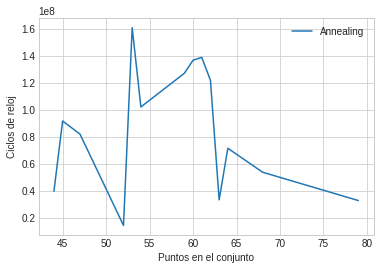
\includegraphics[scale=0.6]{exercise5/annealing3.png}
\end{figure}

Como era de esperar, el gráfico muestra un comportamiento completamente errático por parte del algoritmo. Esto se debe a los tres factores nombrados en la explicación del algoritmo: la solución inicial, la forma del plano de la distancia total de las soluciones y el azar.



\subsubsubsection{Medición en base a distribución del grafo}


En este caso, se espera que haya una diferencia dado que parte de una solución incial ya calculada que cuenta con una diferencia entre cada dataset. Sin embargo, dado que el azar, por ejemplo, es un factor del desarrollo del algoritmo, no sorprendería que en el tiempo final ambos casos tengan un tiempo parecido.

\begin{figure}[H]
	\centering
	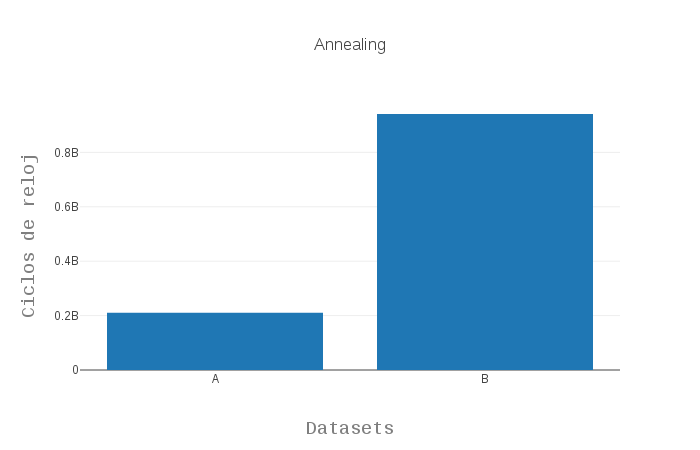
\includegraphics[scale=0.4]{exercise5/annealingType.png}
\end{figure}


Se cumplió con la suposición inicial en la que la diferencia de performance es notable.